
\section{Lake at rest with an immersed bump}

This is a simple test if the method is well-balanced. 
The initial condition is a lake at rest with water depth $0.5$. The topography is
\begin{equation}
z(x)= \left\{ \begin{array}{ll}
 0.2-0.05\left(x-10\right)^2& ~\textrm{if}\quad 8 \leq x \leq 12\,,\\
 0& ~\textrm{otherwise,}\\
\end{array} \right.
\end{equation}
The analytical solution is obviously a lake at rest, that is, $w=0.5$ and $u=v=0$.


\subsection{Results}

Setting up the boundaries to be reflective, we should see excellent agreement between the analytical and numerical solutions if the method is well-balanced. Some oscillations may occur, but if the method is well-balanced, they should be very close to the order of the machine precision. The following three figures show the stage, $x$-momentum, and $x$-velocity after running \anuga{} for some time.

\begin{figure}
\begin{center}
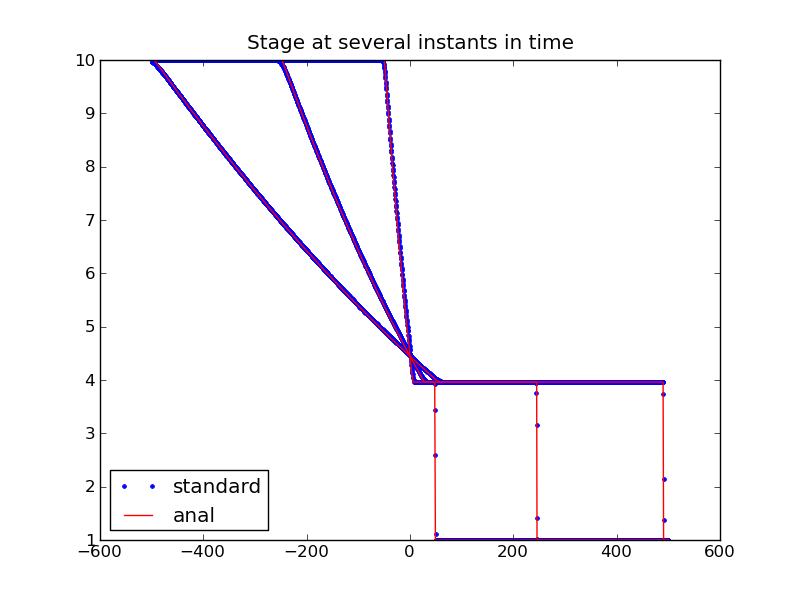
\includegraphics[width=0.9\textwidth]{stage_plot.png}
\end{center}
\caption{Stage results}
\end{figure}


\begin{figure}
\begin{center}
\includegraphics[width=0.9\textwidth]{xmom_plot.png}
\end{center}
\caption{Xmomentum results}
\end{figure}


\begin{figure}
\begin{center}
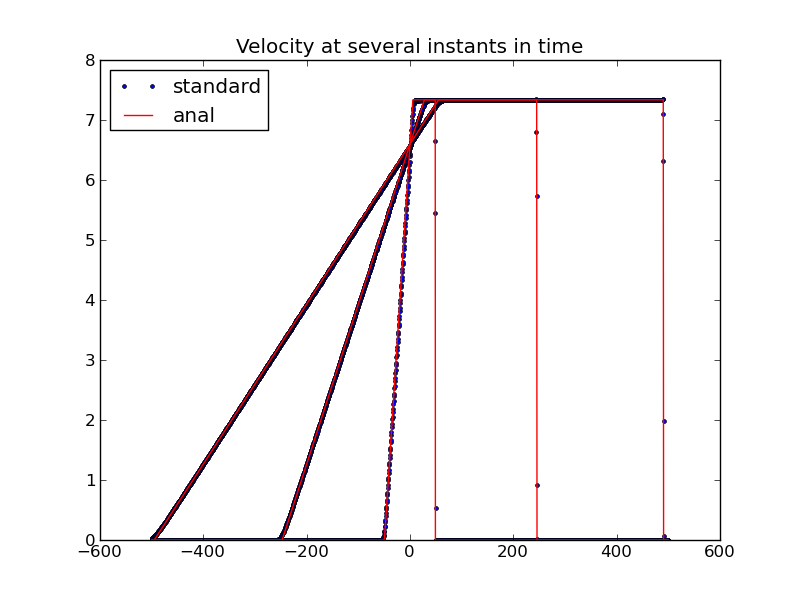
\includegraphics[width=0.9\textwidth]{xvel_plot.png}
\end{center}
\caption{Xvelocity results}
\end{figure}


\endinput
